\tocless\subsection{Objective}
As we can see in section \ref{slidingWindow}, using sliding windows to classify many sections
of an image, there were some cases where some unexpected predictions were made.
Due to this, the decision was made to analyse the effect the background of the
image on its classification. The sliding window code was then ran on a new
image. This new image was the same fruit bowl as used previously but the
background was filled in as white as per Figure \ref{fig:filledFruit}.

\begin{figure}[h]
\centering
    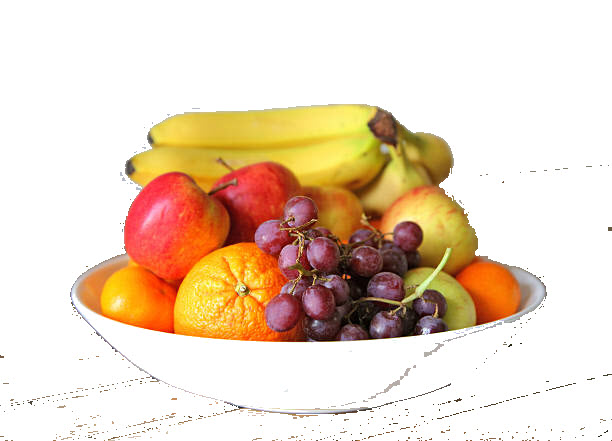
\includegraphics[scale=0.75]{fruitFillBg}
    \caption{Bowl of fruit with background removed}
    \label{fig:filledFruit}
\end{figure}

\begin{table}[h]
    \centering
    \caption{Comparison of fruit image sliding window results with and without
    background}
    \label{comparisionFruitTable}
    \begin{tabular}{|l|l|l|l|p{1.25cm}|p{1.25cm}|p{2cm}|}
    \hline
        \textbf{Food type} & \textbf{Grid} & \textbf{Row} & \textbf{Column} & \textbf{White Grid} & \textbf{White Row} & \textbf{White Column} \\ \hline
        Apple     & 5    & 1   & 3      & 10          & 0          & 4
        \\ \hline
        Banana    & 1    & 0   & 1      & 0           & 0          & 0
        \\ \hline
        Grape     & 4    & 0   & 0      & 1           & 0          & 1
        \\ \hline
        Orange    & 5    & 0   & 0      & 3           & 0          & 0
        \\ \hline
        Other     & 0    & 3   & 1      & 1           & 4          & 0  \\ \hline           
    \end{tabular}
\end{table}

\tocless\subsection{Results}
\tocless\subsubsection{Grid}
For grid-based sliding window approach, the results turned out to be less
successful than with the background. In this experiment, fourteen out of fifteen
of top-1 classification were of an expected food type rather than fifteen out of
fifteen with the background present. We expected the food types of apple,
orange, grape and banana to appear in this image but while a banana was detected
to a top-5 accuracy on a few occasions it was never predicted to a top-1
accuracy. The contrast between the image results can be seen in Table
\ref{comparisionFruitTable}.

\tocless\subsubsection{Row}
The row-based sliding window again had worse result than its counterpart, with
zero out of four correct classifications as opposed to one. In this case, an
orange appeared at top-5 accuracy once. The most common prediction was ice-cream
which appeared at top-1 accuracy in three out of four instances.

\tocless\subsubsection{Column}
In contrast to our previous two methods of sliding window, this method
outperformed its counterpart with correct predictions of all five windows while
before we only had four out of five. In this experiment, an apple was predicted
four times and a grape once, with all correct fruits appearing to top-5
accuracy.

\tocless\subsection{Analysis}
Surprisingly, removing the background of the image reduced the prediction
accuracy.
Many white foods were classified instead which makes sense due
the impact of colour expected.
